\chapter{Result and Analysis}

\section{Parameters for comparison}
3 kinds of graphs have been primarily used to evaluate the performance of our proposed  algorithm which are 

\begin{itemize}
    \item \textbf{Key Generation Time} : This represents the amount of time the algorithm takes to generate the public key and the secret key based on the access policy size .
 \item \textbf{Encryption Time} : This represents the amount of time it takes to encrypt a given generic text file which can be examined while looking at our code .
  \item \textbf{Decryption Time} : This represents the amount of time it takes to decrypt a given encrypted document so as to get the original information.
\end{itemize}

\subsection{Range Value Comparison}
Theoretical calculations and graphs also have been provided along with our own benchmarks so as to show case the efficiencies of our algorithm. The most important graph can be the key generation symmetric and decryption time vs the actual range because our whole solution is about optimizing the extremely big numerical ranges compared to the generic implementation of CP-ABE which are extremely slow and memory hogging for moderately big values of numbers. Now lets’ observe the graphs obtained for extremely large value of ranges which were implemented in the access policy of the form  \(x < range1 \)  and   \(x > range2\) .

\begin{figure}[h]
    \centering
    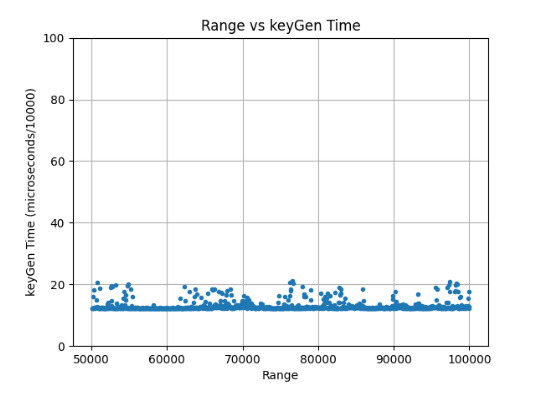
\includegraphics[width=0.75\linewidth]{Images/RangeVsKeyGen.jpeg}
    \caption{Range vs Time Taken For key generation}
    \label{fig:enter-label}
\end{figure}


\begin{figure}[h]
    \centering
    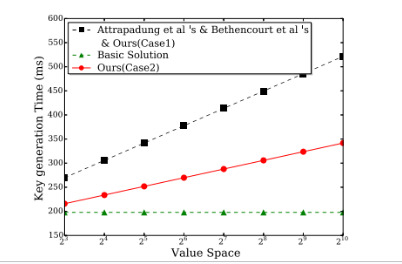
\includegraphics[width=0.75\linewidth]{Images/RangeVsKeyGenTheoritical.jpeg}
    \caption{Range vs Time Taken For key generation Theoritical}
    \label{fig:enter-label}
\end{figure}

An extremely slow growing almost constant \(O(1)\) complexity is observed in the time consumption for the keyGen algorithm which proves that our algorithm is way faster than the generic implementation of range queries for CP-ABE which is \(O(N)\) in nature which blows up very quickly in terms of memory as well as time required for calculations.
This almost constant time complexity is in line with the theoretical calculations that were proved in the paper that was used for reference.


\subsection{Access Length Comparison}
We observe that the time taken for Key Generation remains pretty much constant irrespective of the access policy length which is in line with our assumption that irrespective of the fact that how big the number of attributes get the growth is extremely slow approximately log (n) or barely constant. 
Similar graphs can be drawn for encryption and decryption time which can be used to draw some conclusions about the various optimisation techniques that can be used in the decrypting process which can be observed in the next page.
In case of attribute length as  a parameter which represents the number of parameters present in the user who is trying to decrypt the encrypted file and linearly increasing but stable relationship is observed between the key generation time and number of parameters in Attribute for a given user.

\begin{figure}[h]
    \centering
    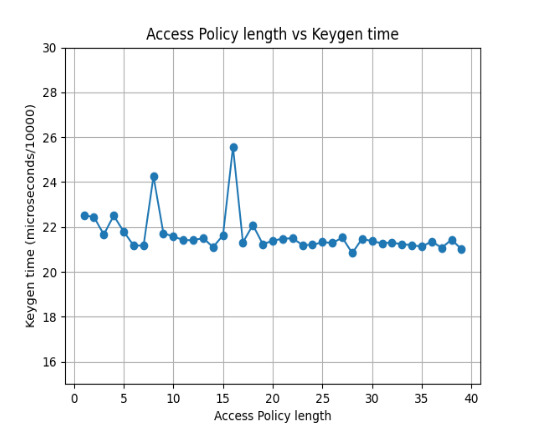
\includegraphics[width=0.75\linewidth]{Images/AccessPolicyLengthVsKeyGenTime.jpeg}
 
    \caption{Access Policy Length vs Time Taken For key generation }
    \label{fig:enter-label}
\end{figure}


\begin{figure}
    \centering
    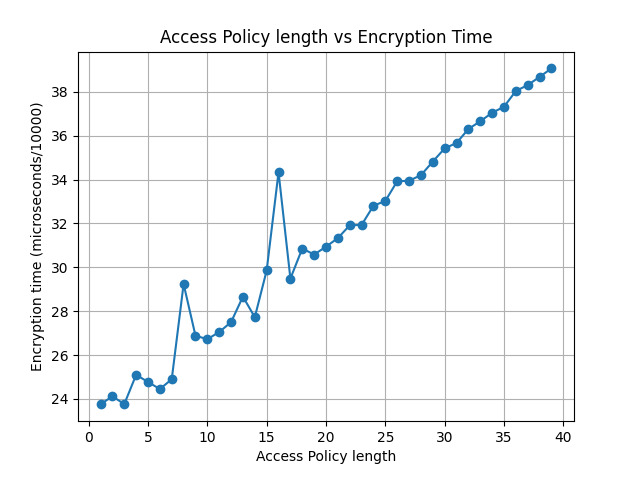
\includegraphics[width=0.75\linewidth]{Images/AccessPolicyLengthVsEncryptionTime.jpeg}
    \caption{Access Policy Length vs Encryption Time }
    \label{fig:enter-label}
\end{figure}


\begin{figure}
    \centering
    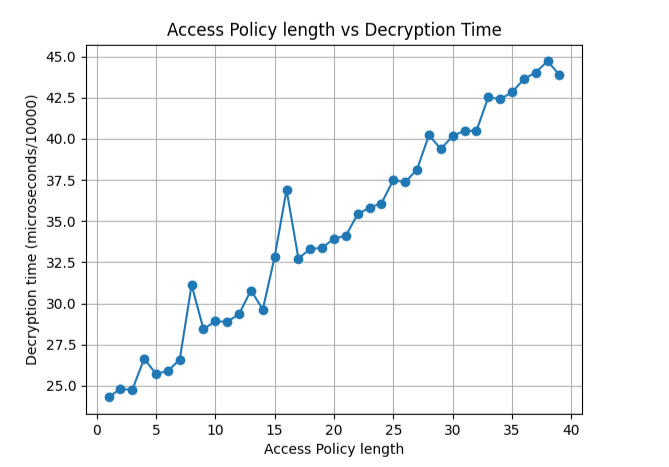
\includegraphics[width=0.75\linewidth]{Images/AccessPolicyVsDecryptionTime.jpeg}
    \caption{Access Policy Length vs Encryption Time }
    \label{fig:enter-label}
\end{figure}


\subsection{Attribute Length Comparison}
In case of attribute length as  a parameter which represents the number of parameters present in the user who is trying to decrypt the encrypted file and linearly increasing but stable relationship is observed between the key generation time and number of parameters in Attribute for a given user.
Some uniformity is observed in the encryption algorithm where as some non linearity can be observed in the decryption algorithm which is due to varying level of optimisations being performed with the given access structure and given attribute properties array for the user attempting to decrypt the file.
Some uniformity is observed in the encryption algorithm where as some non linearity can be observed in the decryption algorithm which is due to varying level of optimisations being performed with the given access structure and given attribute properties array for the user attempting to decrypt the file.

\begin{figure}[h]
    \centering
    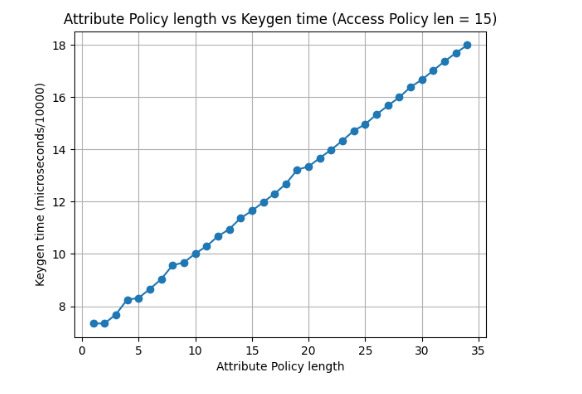
\includegraphics[width=0.75\linewidth]{Images/AttributeLenghtVsKeyGen.jpeg}
 
    \caption{Attribute Policy Length vs Time Taken For key generation }
    \label{fig:enter-label}
\end{figure}


\begin{figure}
    \centering
    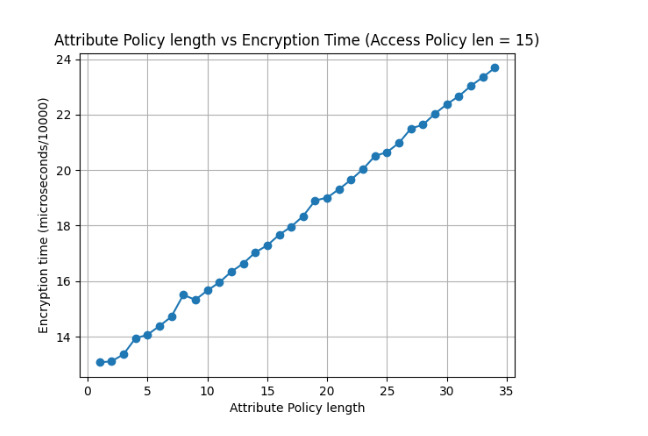
\includegraphics[width=0.75\linewidth]{Images/AttributeLenghtVsEncryptionTime.jpeg}
    \caption{Attribute Policy Length vs Encryption Time }
    \label{fig:enter-label}
\end{figure}


\begin{figure}
    \centering
    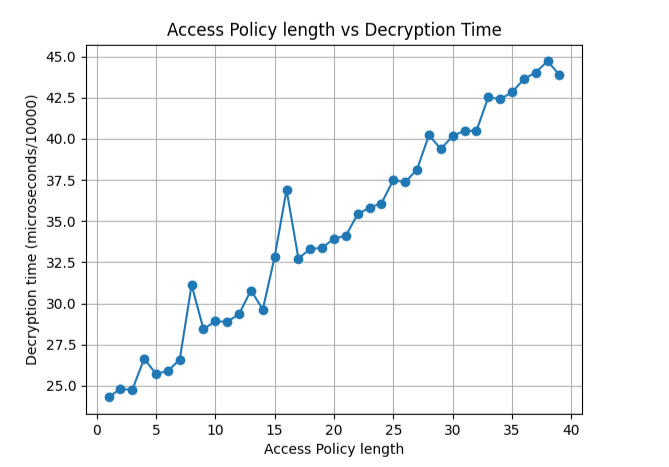
\includegraphics[width=0.75\linewidth]{Images/AccessPolicyVsDecryptionTime.jpeg}
    \caption{Attribute Policy Length vs Encryption Time }
    \label{fig:enter-label}
\end{figure}
